\documentclass[1p]{elsarticle_modified}
%\bibliographystyle{elsarticle-num}

%\usepackage[colorlinks]{hyperref}
%\usepackage{abbrmath_seonhwa} %\Abb, \Ascr, \Acal ,\Abf, \Afrak
\usepackage{amsfonts}
\usepackage{amssymb}
\usepackage{amsmath}
\usepackage{amsthm}
\usepackage{scalefnt}
\usepackage{amsbsy}
\usepackage{kotex}
\usepackage{caption}
\usepackage{subfig}
\usepackage{color}
\usepackage{graphicx}
\usepackage{xcolor} %% white, black, red, green, blue, cyan, magenta, yellow
\usepackage{float}
\usepackage{setspace}
\usepackage{hyperref}

\usepackage{tikz}
\usetikzlibrary{arrows}

\usepackage{multirow}
\usepackage{array} % fixed length table
\usepackage{hhline}

%%%%%%%%%%%%%%%%%%%%%
\makeatletter
\renewcommand*\env@matrix[1][\arraystretch]{%
	\edef\arraystretch{#1}%
	\hskip -\arraycolsep
	\let\@ifnextchar\new@ifnextchar
	\array{*\c@MaxMatrixCols c}}
\makeatother %https://tex.stackexchange.com/questions/14071/how-can-i-increase-the-line-spacing-in-a-matrix
%%%%%%%%%%%%%%%

\usepackage[normalem]{ulem}

\newcommand{\msout}[1]{\ifmmode\text{\sout{\ensuremath{#1}}}\else\sout{#1}\fi}
%SOURCE: \msout is \stkout macro in https://tex.stackexchange.com/questions/20609/strikeout-in-math-mode

\newcommand{\cancel}[1]{
	\ifmmode
	{\color{red}\msout{#1}}
	\else
	{\color{red}\sout{#1}}
	\fi
}

\newcommand{\add}[1]{
	{\color{blue}\uwave{#1}}
}

\newcommand{\replace}[2]{
	\ifmmode
	{\color{red}\msout{#1}}{\color{blue}\uwave{#2}}
	\else
	{\color{red}\sout{#1}}{\color{blue}\uwave{#2}}
	\fi
}

\newcommand{\Sol}{\mathcal{S}} %segment
\newcommand{\D}{D} %diagram
\newcommand{\A}{\mathcal{A}} %arc


%%%%%%%%%%%%%%%%%%%%%%%%%%%%%5 test

\def\sl{\operatorname{\textup{SL}}(2,\Cbb)}
\def\psl{\operatorname{\textup{PSL}}(2,\Cbb)}
\def\quan{\mkern 1mu \triangleright \mkern 1mu}

\theoremstyle{definition}
\newtheorem{thm}{Theorem}[section]
\newtheorem{prop}[thm]{Proposition}
\newtheorem{lem}[thm]{Lemma}
\newtheorem{ques}[thm]{Question}
\newtheorem{cor}[thm]{Corollary}
\newtheorem{defn}[thm]{Definition}
\newtheorem{exam}[thm]{Example}
\newtheorem{rmk}[thm]{Remark}
\newtheorem{alg}[thm]{Algorithm}

\newcommand{\I}{\sqrt{-1}}
\begin{document}

%\begin{frontmatter}
%
%\title{Boundary parabolic representations of knots up to 8 crossings}
%
%%% Group authors per affiliation:
%\author{Yunhi Cho} 
%\address{Department of Mathematics, University of Seoul, Seoul, Korea}
%\ead{yhcho@uos.ac.kr}
%
%
%\author{Seonhwa Kim} %\fnref{s_kim}}
%\address{Center for Geometry and Physics, Institute for Basic Science, Pohang, 37673, Korea}
%\ead{ryeona17@ibs.re.kr}
%
%\author{Hyuk Kim}
%\address{Department of Mathematical Sciences, Seoul National University, Seoul 08826, Korea}
%\ead{hyukkim@snu.ac.kr}
%
%\author{Seokbeom Yoon}
%\address{Department of Mathematical Sciences, Seoul National University, Seoul, 08826,  Korea}
%\ead{sbyoon15@snu.ac.kr}
%
%\begin{abstract}
%We find all boundary parabolic representation of knots up to 8 crossings.
%
%\end{abstract}
%\begin{keyword}
%    \MSC[2010] 57M25 
%\end{keyword}
%
%\end{frontmatter}

%\linenumbers
%\tableofcontents
%
\newcommand\colored[1]{\textcolor{white}{\rule[-0.35ex]{0.8em}{1.4ex}}\kern-0.8em\color{red} #1}%
%\newcommand\colored[1]{\textcolor{white}{ #1}\kern-2.17ex	\textcolor{white}{ #1}\kern-1.81ex	\textcolor{white}{ #1}\kern-2.15ex\color{red}#1	}

{\Large $\underline{12a_{1111}~(K12a_{1111})}$}

\setlength{\tabcolsep}{10pt}
\renewcommand{\arraystretch}{1.6}
\vspace{1cm}\begin{tabular}{m{100pt}>{\centering\arraybackslash}m{274pt}}
\multirow{5}{120pt}{
	\centering
	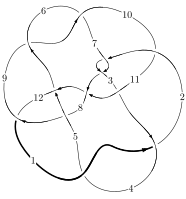
\includegraphics[width=112pt]{../../../GIT/diagram.site/Diagrams/png/1912_12a_1111.png}\\
\ \ \ A knot diagram\footnotemark}&
\allowdisplaybreaks
\textbf{Linearized knot diagam} \\
\cline{2-2}
 &
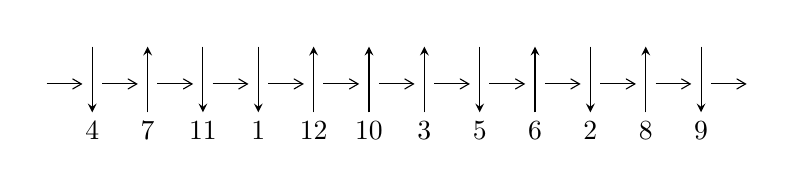
\begin{tikzpicture}[x=20pt, y=17pt]
	% nodes
	\node (C0) at (0, 0) {};
	\node (C1) at (1, 0) {};
	\node (C1U) at (1, +1) {};
	\node (C1D) at (1, -1) {4};

	\node (C2) at (2, 0) {};
	\node (C2U) at (2, +1) {};
	\node (C2D) at (2, -1) {7};

	\node (C3) at (3, 0) {};
	\node (C3U) at (3, +1) {};
	\node (C3D) at (3, -1) {11};

	\node (C4) at (4, 0) {};
	\node (C4U) at (4, +1) {};
	\node (C4D) at (4, -1) {1};

	\node (C5) at (5, 0) {};
	\node (C5U) at (5, +1) {};
	\node (C5D) at (5, -1) {12};

	\node (C6) at (6, 0) {};
	\node (C6U) at (6, +1) {};
	\node (C6D) at (6, -1) {10};

	\node (C7) at (7, 0) {};
	\node (C7U) at (7, +1) {};
	\node (C7D) at (7, -1) {3};

	\node (C8) at (8, 0) {};
	\node (C8U) at (8, +1) {};
	\node (C8D) at (8, -1) {5};

	\node (C9) at (9, 0) {};
	\node (C9U) at (9, +1) {};
	\node (C9D) at (9, -1) {6};

	\node (C10) at (10, 0) {};
	\node (C10U) at (10, +1) {};
	\node (C10D) at (10, -1) {2};

	\node (C11) at (11, 0) {};
	\node (C11U) at (11, +1) {};
	\node (C11D) at (11, -1) {8};

	\node (C12) at (12, 0) {};
	\node (C12U) at (12, +1) {};
	\node (C12D) at (12, -1) {9};
	\node (C13) at (13, 0) {};

	% arrows
	\draw[->,>={angle 60}]
	(C0) edge (C1) (C1) edge (C2) (C2) edge (C3) (C3) edge (C4) (C4) edge (C5) (C5) edge (C6) (C6) edge (C7) (C7) edge (C8) (C8) edge (C9) (C9) edge (C10) (C10) edge (C11) (C11) edge (C12) (C12) edge (C13) ;	\draw[->,>=stealth]
	(C1U) edge (C1D) (C2D) edge (C2U) (C3U) edge (C3D) (C4U) edge (C4D) (C5D) edge (C5U) (C6D) edge (C6U) (C7D) edge (C7U) (C8U) edge (C8D) (C9D) edge (C9U) (C10U) edge (C10D) (C11D) edge (C11U) (C12U) edge (C12D) ;
	\end{tikzpicture} \\
\hhline{~~} \\& 
\textbf{Solving Sequence} \\ \cline{2-2} 
 &
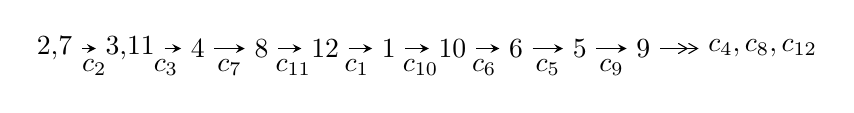
\begin{tikzpicture}[x=23pt, y=7pt]
	% node
	\node (A0) at (-1/8, 0) {2,7};
	\node (A1) at (17/16, 0) {3,11};
	\node (A2) at (17/8, 0) {4};
	\node (A3) at (25/8, 0) {8};
	\node (A4) at (33/8, 0) {12};
	\node (A5) at (41/8, 0) {1};
	\node (A6) at (49/8, 0) {10};
	\node (A7) at (57/8, 0) {6};
	\node (A8) at (65/8, 0) {5};
	\node (A9) at (73/8, 0) {9};
	\node (C1) at (1/2, -1) {$c_{2}$};
	\node (C2) at (13/8, -1) {$c_{3}$};
	\node (C3) at (21/8, -1) {$c_{7}$};
	\node (C4) at (29/8, -1) {$c_{11}$};
	\node (C5) at (37/8, -1) {$c_{1}$};
	\node (C6) at (45/8, -1) {$c_{10}$};
	\node (C7) at (53/8, -1) {$c_{6}$};
	\node (C8) at (61/8, -1) {$c_{5}$};
	\node (C9) at (69/8, -1) {$c_{9}$};
	\node (A10) at (11, 0) {$c_{4},c_{8},c_{12}$};

	% edge
	\draw[->,>=stealth]	
	(A0) edge (A1) (A1) edge (A2) (A2) edge (A3) (A3) edge (A4) (A4) edge (A5) (A5) edge (A6) (A6) edge (A7) (A7) edge (A8) (A8) edge (A9) ;
	\draw[->>,>={angle 60}]	
	(A9) edge (A10);
\end{tikzpicture} \\ 

\end{tabular} \\

\footnotetext{
The image of knot diagram is generated by the software ``\textbf{Draw programme}" developed by Andrew Bartholomew(\url{http://www.layer8.co.uk/maths/draw/index.htm\#Running-draw}), where we modified some parts for our purpose(\url{https://github.com/CATsTAILs/LinksPainter}).
}\phantom \\ \newline 
\centering \textbf{Ideals for irreducible components\footnotemark of $X_{\text{par}}$} 
 
\begin{align*}
I^u_{1}&=\langle 
6.44358\times10^{663} u^{142}-3.78775\times10^{662} u^{141}+\cdots+6.82477\times10^{666} b+1.57113\times10^{666},\\
\phantom{I^u_{1}}&\phantom{= \langle  }3.65254\times10^{666} u^{142}-5.30227\times10^{666} u^{141}+\cdots+7.02951\times10^{668} a+1.55949\times10^{669},\\
\phantom{I^u_{1}}&\phantom{= \langle  }u^{143}- u^{142}+\cdots+386 u+206\rangle \\
I^u_{2}&=\langle 
2.25450\times10^{32} u^{39}+6.59613\times10^{31} u^{38}+\cdots+9.63661\times10^{32} b+2.18292\times10^{33},\\
\phantom{I^u_{2}}&\phantom{= \langle  }1.16107\times10^{33} u^{39}-1.36968\times10^{33} u^{38}+\cdots+1.92732\times10^{33} a+1.04728\times10^{34},\;u^{40}-13 u^{38}+\cdots+10 u+2\rangle \\
\\
\end{align*}
\raggedright * 2 irreducible components of $\dim_{\mathbb{C}}=0$, with total 183 representations.\\
\footnotetext{All coefficients of polynomials are rational numbers. But the coefficients are sometimes approximated in decimal forms when there is not enough margin.}
\newpage
\renewcommand{\arraystretch}{1}
\centering \section*{I. $I^u_{1}= \langle 6.44\times10^{663} u^{142}-3.79\times10^{662} u^{141}+\cdots+6.82\times10^{666} b+1.57\times10^{666},\;3.65\times10^{666} u^{142}-5.30\times10^{666} u^{141}+\cdots+7.03\times10^{668} a+1.56\times10^{669},\;u^{143}- u^{142}+\cdots+386 u+206 \rangle$}
\flushleft \textbf{(i) Arc colorings}\\
\begin{tabular}{m{7pt} m{180pt} m{7pt} m{180pt} }
\flushright $a_{2}=$&$\begin{pmatrix}1\\0\end{pmatrix}$ \\
\flushright $a_{7}=$&$\begin{pmatrix}0\\u\end{pmatrix}$ \\
\flushright $a_{3}=$&$\begin{pmatrix}1\\- u^2\end{pmatrix}$ \\
\flushright $a_{11}=$&$\begin{pmatrix}-0.00519601 u^{142}+0.00754286 u^{141}+\cdots+4.73232 u-2.21849\\-0.000944146 u^{142}+0.0000555000 u^{141}+\cdots-4.11931 u-0.230210\end{pmatrix}$ \\
\flushright $a_{4}=$&$\begin{pmatrix}0.00264122 u^{142}-0.00202716 u^{141}+\cdots+12.5165 u-1.10038\\-0.00174240 u^{142}-0.00124465 u^{141}+\cdots+0.502531 u-0.481627\end{pmatrix}$ \\
\flushright $a_{8}=$&$\begin{pmatrix}u\\- u^3+u\end{pmatrix}$ \\
\flushright $a_{12}=$&$\begin{pmatrix}-0.00555176 u^{142}+0.00903576 u^{141}+\cdots+3.46011 u-2.53093\\-0.000701503 u^{142}+0.0000127943 u^{141}+\cdots-5.02587 u-0.308388\end{pmatrix}$ \\
\flushright $a_{1}=$&$\begin{pmatrix}0.00195969 u^{142}-0.00530041 u^{141}+\cdots-7.01821 u-2.88220\\0.000282759 u^{142}+0.00134612 u^{141}+\cdots+1.62966 u-0.410901\end{pmatrix}$ \\
\flushright $a_{10}=$&$\begin{pmatrix}-0.00614015 u^{142}+0.00759836 u^{141}+\cdots+0.613008 u-2.44871\\-0.000944146 u^{142}+0.0000555000 u^{141}+\cdots-4.11931 u-0.230210\end{pmatrix}$ \\
\flushright $a_{6}=$&$\begin{pmatrix}0.00621299 u^{142}-0.00774462 u^{141}+\cdots-7.23321 u+5.22982\\0.000367164 u^{142}-0.00594574 u^{141}+\cdots+6.69531 u+1.01883\end{pmatrix}$ \\
\flushright $a_{5}=$&$\begin{pmatrix}0.00434444 u^{142}-0.00318853 u^{141}+\cdots+10.6877 u-3.04330\\0.000852588 u^{142}+0.000829582 u^{141}+\cdots+1.86680 u-0.404961\end{pmatrix}$ \\
\flushright $a_{9}=$&$\begin{pmatrix}0.00381391 u^{142}-0.00485688 u^{141}+\cdots-13.7966 u+4.54115\\0.00582786 u^{142}+0.000899180 u^{141}+\cdots-2.10823 u-0.785313\end{pmatrix}$\\&\end{tabular}
\flushleft \textbf{(ii) Obstruction class $= -1$}\\~\\
\flushleft \textbf{(iii) Cusp Shapes $= -0.0323696 u^{142}+0.0169279 u^{141}+\cdots+14.8197 u+8.68835$}\\~\\
\newpage\renewcommand{\arraystretch}{1}
\flushleft \textbf{(iv) u-Polynomials at the component}\newline \\
\begin{tabular}{m{50pt}|m{274pt}}
Crossings & \hspace{64pt}u-Polynomials at each crossing \\
\hline $$\begin{aligned}c_{1},c_{4}\end{aligned}$$&$\begin{aligned}
&u^{143}-9 u^{142}+\cdots-60 u+1
\end{aligned}$\\
\hline $$\begin{aligned}c_{2},c_{7}\end{aligned}$$&$\begin{aligned}
&u^{143}+u^{142}+\cdots+386 u-206
\end{aligned}$\\
\hline $$\begin{aligned}c_{3}\end{aligned}$$&$\begin{aligned}
&u^{143}+5 u^{142}+\cdots-201714210 u+12357493
\end{aligned}$\\
\hline $$\begin{aligned}c_{5}\end{aligned}$$&$\begin{aligned}
&u^{143}-4 u^{142}+\cdots-117392 u-5947
\end{aligned}$\\
\hline $$\begin{aligned}c_{6},c_{9}\end{aligned}$$&$\begin{aligned}
&u^{143}-9 u^{142}+\cdots-29761 u+6317
\end{aligned}$\\
\hline $$\begin{aligned}c_{8}\end{aligned}$$&$\begin{aligned}
&u^{143}-3 u^{142}+\cdots+165724 u+28690
\end{aligned}$\\
\hline $$\begin{aligned}c_{10}\end{aligned}$$&$\begin{aligned}
&u^{143}+3 u^{142}+\cdots-6317830 u+1664477
\end{aligned}$\\
\hline $$\begin{aligned}c_{11}\end{aligned}$$&$\begin{aligned}
&u^{143}+5 u^{142}+\cdots+452720672761 u-54947494499
\end{aligned}$\\
\hline $$\begin{aligned}c_{12}\end{aligned}$$&$\begin{aligned}
&u^{143}+2 u^{142}+\cdots+393169 u-36221
\end{aligned}$\\
\hline
\end{tabular}\\~\\
\newpage\renewcommand{\arraystretch}{1}
\flushleft \textbf{(v) Riley Polynomials at the component}\newline \\
\begin{tabular}{m{50pt}|m{274pt}}
Crossings & \hspace{64pt}Riley Polynomials at each crossing \\
\hline $$\begin{aligned}c_{1},c_{4}\end{aligned}$$&$\begin{aligned}
&y^{143}+133 y^{142}+\cdots-532 y-1
\end{aligned}$\\
\hline $$\begin{aligned}c_{2},c_{7}\end{aligned}$$&$\begin{aligned}
&y^{143}-107 y^{142}+\cdots-4268 y-42436
\end{aligned}$\\
\hline $$\begin{aligned}c_{3}\end{aligned}$$&$\begin{aligned}
&y^{143}+61 y^{142}+\cdots+345432706394200 y-152707633245049
\end{aligned}$\\
\hline $$\begin{aligned}c_{5}\end{aligned}$$&$\begin{aligned}
&y^{143}-36 y^{142}+\cdots+1571191116 y-35366809
\end{aligned}$\\
\hline $$\begin{aligned}c_{6},c_{9}\end{aligned}$$&$\begin{aligned}
&y^{143}-147 y^{142}+\cdots-2851394811 y-39904489
\end{aligned}$\\
\hline $$\begin{aligned}c_{8}\end{aligned}$$&$\begin{aligned}
&y^{143}+31 y^{142}+\cdots-38326890024 y-823116100
\end{aligned}$\\
\hline $$\begin{aligned}c_{10}\end{aligned}$$&$\begin{aligned}
&y^{143}+77 y^{142}+\cdots-1249728511533410 y-2770483683529
\end{aligned}$\\
\hline $$\begin{aligned}c_{11}\end{aligned}$$&$\begin{aligned}
&y^{143}-107 y^{142}+\cdots-1.85\times10^{23} y-3.02\times10^{21}
\end{aligned}$\\
\hline $$\begin{aligned}c_{12}\end{aligned}$$&$\begin{aligned}
&y^{143}+50 y^{142}+\cdots-57389804335 y-1311960841
\end{aligned}$\\
\hline
\end{tabular}\\~\\
\newpage\flushleft \textbf{(vi) Complex Volumes and Cusp Shapes}
$$\begin{array}{c|c|c}  
\text{Solutions to }I^u_{1}& \I (\text{vol} + \sqrt{-1}CS) & \text{Cusp shape}\\
 \hline 
\begin{aligned}
u &= \phantom{-}0.063249 + 0.982291 I \\
a &= \phantom{-}0.063883 - 0.226508 I \\
b &= \phantom{-}0.508736 + 0.372416 I\end{aligned}
 & -1.21642 - 3.83650 I & \phantom{-0.000000 } 0 \\ \hline\begin{aligned}
u &= \phantom{-}0.063249 - 0.982291 I \\
a &= \phantom{-}0.063883 + 0.226508 I \\
b &= \phantom{-}0.508736 - 0.372416 I\end{aligned}
 & -1.21642 + 3.83650 I & \phantom{-0.000000 } 0 \\ \hline\begin{aligned}
u &= \phantom{-}0.955376 + 0.175175 I \\
a &= \phantom{-}0.20674 - 1.62306 I \\
b &= -0.514277 + 0.891938 I\end{aligned}
 & -0.19601 + 2.73913 I & \phantom{-0.000000 } 0 \\ \hline\begin{aligned}
u &= \phantom{-}0.955376 - 0.175175 I \\
a &= \phantom{-}0.20674 + 1.62306 I \\
b &= -0.514277 - 0.891938 I\end{aligned}
 & -0.19601 - 2.73913 I & \phantom{-0.000000 } 0 \\ \hline\begin{aligned}
u &= \phantom{-}0.726188 + 0.618520 I \\
a &= \phantom{-}0.112078 - 0.271226 I \\
b &= \phantom{-}0.774241 - 0.065819 I\end{aligned}
 & \phantom{-}0.91442 + 6.37781 I & \phantom{-0.000000 } 0 \\ \hline\begin{aligned}
u &= \phantom{-}0.726188 - 0.618520 I \\
a &= \phantom{-}0.112078 + 0.271226 I \\
b &= \phantom{-}0.774241 + 0.065819 I\end{aligned}
 & \phantom{-}0.91442 - 6.37781 I & \phantom{-0.000000 } 0 \\ \hline\begin{aligned}
u &= \phantom{-}0.930195 + 0.112377 I \\
a &= -3.52277 - 1.80840 I \\
b &= \phantom{-}0.005674 + 0.466916 I\end{aligned}
 & \phantom{-}7.99535 + 0.15590 I & \phantom{-0.000000 } 0 \\ \hline\begin{aligned}
u &= \phantom{-}0.930195 - 0.112377 I \\
a &= -3.52277 + 1.80840 I \\
b &= \phantom{-}0.005674 - 0.466916 I\end{aligned}
 & \phantom{-}7.99535 - 0.15590 I & \phantom{-0.000000 } 0 \\ \hline\begin{aligned}
u &= \phantom{-}0.381192 + 0.854280 I \\
a &= -1.068870 - 0.053312 I \\
b &= \phantom{-}0.51243 + 1.39432 I\end{aligned}
 & \phantom{-}6.44515 - 4.49680 I & \phantom{-0.000000 } 0 \\ \hline\begin{aligned}
u &= \phantom{-}0.381192 - 0.854280 I \\
a &= -1.068870 + 0.053312 I \\
b &= \phantom{-}0.51243 - 1.39432 I\end{aligned}
 & \phantom{-}6.44515 + 4.49680 I & \phantom{-0.000000 } 0\\
 \hline 
 \end{array}$$\newpage$$\begin{array}{c|c|c}  
\text{Solutions to }I^u_{1}& \I (\text{vol} + \sqrt{-1}CS) & \text{Cusp shape}\\
 \hline 
\begin{aligned}
u &= -1.072310 + 0.175968 I \\
a &= -0.39712 - 2.28045 I \\
b &= \phantom{-}0.55071 + 1.62247 I\end{aligned}
 & \phantom{-}3.98724 - 5.90791 I & \phantom{-0.000000 } 0 \\ \hline\begin{aligned}
u &= -1.072310 - 0.175968 I \\
a &= -0.39712 + 2.28045 I \\
b &= \phantom{-}0.55071 - 1.62247 I\end{aligned}
 & \phantom{-}3.98724 + 5.90791 I & \phantom{-0.000000 } 0 \\ \hline\begin{aligned}
u &= -1.101400 + 0.087788 I \\
a &= \phantom{-}0.61298 + 1.66555 I \\
b &= -0.224702 - 0.818323 I\end{aligned}
 & \phantom{-}1.245020 - 0.471467 I & \phantom{-0.000000 } 0 \\ \hline\begin{aligned}
u &= -1.101400 - 0.087788 I \\
a &= \phantom{-}0.61298 - 1.66555 I \\
b &= -0.224702 + 0.818323 I\end{aligned}
 & \phantom{-}1.245020 + 0.471467 I & \phantom{-0.000000 } 0 \\ \hline\begin{aligned}
u &= -0.367676 + 0.811167 I \\
a &= \phantom{-}0.783968 + 0.422049 I \\
b &= -0.383251 + 0.925400 I\end{aligned}
 & \phantom{-}1.98662 + 2.18393 I & \phantom{-0.000000 } 0 \\ \hline\begin{aligned}
u &= -0.367676 - 0.811167 I \\
a &= \phantom{-}0.783968 - 0.422049 I \\
b &= -0.383251 - 0.925400 I\end{aligned}
 & \phantom{-}1.98662 - 2.18393 I & \phantom{-0.000000 } 0 \\ \hline\begin{aligned}
u &= \phantom{-}0.675904 + 0.579161 I \\
a &= -0.227068 + 0.923405 I \\
b &= -0.0231895 - 0.0517523 I\end{aligned}
 & \phantom{-}0.91339 - 2.14644 I & \phantom{-0.000000 } 0 \\ \hline\begin{aligned}
u &= \phantom{-}0.675904 - 0.579161 I \\
a &= -0.227068 - 0.923405 I \\
b &= -0.0231895 + 0.0517523 I\end{aligned}
 & \phantom{-}0.91339 + 2.14644 I & \phantom{-0.000000 } 0 \\ \hline\begin{aligned}
u &= -0.438458 + 0.767054 I \\
a &= -0.144781 - 0.508785 I \\
b &= \phantom{-}0.718464 + 0.514134 I\end{aligned}
 & \phantom{-}3.41792 - 2.89335 I & \phantom{-0.000000 } 0 \\ \hline\begin{aligned}
u &= -0.438458 - 0.767054 I \\
a &= -0.144781 + 0.508785 I \\
b &= \phantom{-}0.718464 - 0.514134 I\end{aligned}
 & \phantom{-}3.41792 + 2.89335 I & \phantom{-0.000000 } 0\\
 \hline 
 \end{array}$$\newpage$$\begin{array}{c|c|c}  
\text{Solutions to }I^u_{1}& \I (\text{vol} + \sqrt{-1}CS) & \text{Cusp shape}\\
 \hline 
\begin{aligned}
u &= -1.112580 + 0.175274 I \\
a &= \phantom{-}0.22479 - 2.08448 I \\
b &= \phantom{-}0.026394 + 0.583340 I\end{aligned}
 & \phantom{-}3.05740 - 0.82586 I & \phantom{-0.000000 } 0 \\ \hline\begin{aligned}
u &= -1.112580 - 0.175274 I \\
a &= \phantom{-}0.22479 + 2.08448 I \\
b &= \phantom{-}0.026394 - 0.583340 I\end{aligned}
 & \phantom{-}3.05740 + 0.82586 I & \phantom{-0.000000 } 0 \\ \hline\begin{aligned}
u &= \phantom{-}0.138732 + 1.135660 I \\
a &= -0.0619898 + 0.1217210 I \\
b &= -0.521109 + 1.211600 I\end{aligned}
 & \phantom{-}9.61783 + 4.35986 I & \phantom{-0.000000 } 0 \\ \hline\begin{aligned}
u &= \phantom{-}0.138732 - 1.135660 I \\
a &= -0.0619898 - 0.1217210 I \\
b &= -0.521109 - 1.211600 I\end{aligned}
 & \phantom{-}9.61783 - 4.35986 I & \phantom{-0.000000 } 0 \\ \hline\begin{aligned}
u &= -0.519039 + 1.020730 I \\
a &= -0.094411 - 0.193102 I \\
b &= \phantom{-}0.287209 - 0.335176 I\end{aligned}
 & -0.60536 - 3.38632 I & \phantom{-0.000000 } 0 \\ \hline\begin{aligned}
u &= -0.519039 - 1.020730 I \\
a &= -0.094411 + 0.193102 I \\
b &= \phantom{-}0.287209 + 0.335176 I\end{aligned}
 & -0.60536 + 3.38632 I & \phantom{-0.000000 } 0 \\ \hline\begin{aligned}
u &= \phantom{-}1.142070 + 0.133955 I \\
a &= -0.89388 - 1.54878 I \\
b &= \phantom{-}0.748829 + 0.894632 I\end{aligned}
 & \phantom{-}7.40438 + 0.58958 I & \phantom{-0.000000 } 0 \\ \hline\begin{aligned}
u &= \phantom{-}1.142070 - 0.133955 I \\
a &= -0.89388 + 1.54878 I \\
b &= \phantom{-}0.748829 - 0.894632 I\end{aligned}
 & \phantom{-}7.40438 - 0.58958 I & \phantom{-0.000000 } 0 \\ \hline\begin{aligned}
u &= -0.056660 + 0.847707 I \\
a &= -0.334580 - 0.292185 I \\
b &= -0.874752 + 0.867142 I\end{aligned}
 & \phantom{-}4.48567 + 8.36278 I & \phantom{-0.000000 } 0 \\ \hline\begin{aligned}
u &= -0.056660 - 0.847707 I \\
a &= -0.334580 + 0.292185 I \\
b &= -0.874752 - 0.867142 I\end{aligned}
 & \phantom{-}4.48567 - 8.36278 I & \phantom{-0.000000 } 0\\
 \hline 
 \end{array}$$\newpage$$\begin{array}{c|c|c}  
\text{Solutions to }I^u_{1}& \I (\text{vol} + \sqrt{-1}CS) & \text{Cusp shape}\\
 \hline 
\begin{aligned}
u &= \phantom{-}0.414095 + 1.094390 I \\
a &= -0.0007776 - 0.1280520 I \\
b &= \phantom{-}0.494924 - 0.982397 I\end{aligned}
 & \phantom{-}8.82654 + 4.52566 I & \phantom{-0.000000 } 0 \\ \hline\begin{aligned}
u &= \phantom{-}0.414095 - 1.094390 I \\
a &= -0.0007776 + 0.1280520 I \\
b &= \phantom{-}0.494924 + 0.982397 I\end{aligned}
 & \phantom{-}8.82654 - 4.52566 I & \phantom{-0.000000 } 0 \\ \hline\begin{aligned}
u &= \phantom{-}1.092630 + 0.421283 I \\
a &= \phantom{-}0.74496 + 2.20624 I \\
b &= \phantom{-}0.43448 - 2.43810 I\end{aligned}
 & \phantom{-}8.68386 + 9.22388 I & \phantom{-0.000000 } 0 \\ \hline\begin{aligned}
u &= \phantom{-}1.092630 - 0.421283 I \\
a &= \phantom{-}0.74496 - 2.20624 I \\
b &= \phantom{-}0.43448 + 2.43810 I\end{aligned}
 & \phantom{-}8.68386 - 9.22388 I & \phantom{-0.000000 } 0 \\ \hline\begin{aligned}
u &= -1.17738\phantom{ +0.000000I} \\
a &= -0.351660\phantom{ +0.000000I} \\
b &= -1.14009\phantom{ +0.000000I}\end{aligned}
 & \phantom{-}4.79177\phantom{ +0.000000I} & \phantom{-0.000000 } 0 \\ \hline\begin{aligned}
u &= \phantom{-}1.170490 + 0.227959 I \\
a &= \phantom{-}0.06674 - 2.50737 I \\
b &= -0.485949 + 0.684127 I\end{aligned}
 & \phantom{-}7.55504 + 0.96536 I & \phantom{-0.000000 } 0 \\ \hline\begin{aligned}
u &= \phantom{-}1.170490 - 0.227959 I \\
a &= \phantom{-}0.06674 + 2.50737 I \\
b &= -0.485949 - 0.684127 I\end{aligned}
 & \phantom{-}7.55504 - 0.96536 I & \phantom{-0.000000 } 0 \\ \hline\begin{aligned}
u &= -1.132050 + 0.389913 I \\
a &= \phantom{-}0.364665 - 1.095350 I \\
b &= \phantom{-}0.480110 + 0.823925 I\end{aligned}
 & \phantom{-}1.69118 - 1.59714 I & \phantom{-0.000000 } 0 \\ \hline\begin{aligned}
u &= -1.132050 - 0.389913 I \\
a &= \phantom{-}0.364665 + 1.095350 I \\
b &= \phantom{-}0.480110 - 0.823925 I\end{aligned}
 & \phantom{-}1.69118 + 1.59714 I & \phantom{-0.000000 } 0 \\ \hline\begin{aligned}
u &= \phantom{-}1.199240 + 0.023932 I \\
a &= \phantom{-}2.03873 + 1.26924 I \\
b &= -3.16106 - 1.40806 I\end{aligned}
 & \phantom{-}11.9989 + 7.9336 I & \phantom{-0.000000 } 0\\
 \hline 
 \end{array}$$\newpage$$\begin{array}{c|c|c}  
\text{Solutions to }I^u_{1}& \I (\text{vol} + \sqrt{-1}CS) & \text{Cusp shape}\\
 \hline 
\begin{aligned}
u &= \phantom{-}1.199240 - 0.023932 I \\
a &= \phantom{-}2.03873 - 1.26924 I \\
b &= -3.16106 + 1.40806 I\end{aligned}
 & \phantom{-}11.9989 - 7.9336 I & \phantom{-0.000000 } 0 \\ \hline\begin{aligned}
u &= \phantom{-}1.203270 + 0.121115 I \\
a &= -0.537471 - 0.335218 I \\
b &= \phantom{-}1.57872 + 0.08308 I\end{aligned}
 & \phantom{-}7.84470 + 2.02497 I & \phantom{-0.000000 } 0 \\ \hline\begin{aligned}
u &= \phantom{-}1.203270 - 0.121115 I \\
a &= -0.537471 + 0.335218 I \\
b &= \phantom{-}1.57872 - 0.08308 I\end{aligned}
 & \phantom{-}7.84470 - 2.02497 I & \phantom{-0.000000 } 0 \\ \hline\begin{aligned}
u &= -1.146450 + 0.390646 I \\
a &= -0.34421 + 1.62819 I \\
b &= -0.78616 - 1.72700 I\end{aligned}
 & \phantom{-}4.47571 - 6.67031 I & \phantom{-0.000000 } 0 \\ \hline\begin{aligned}
u &= -1.146450 - 0.390646 I \\
a &= -0.34421 - 1.62819 I \\
b &= -0.78616 + 1.72700 I\end{aligned}
 & \phantom{-}4.47571 + 6.67031 I & \phantom{-0.000000 } 0 \\ \hline\begin{aligned}
u &= -0.647983 + 0.435098 I \\
a &= \phantom{-}0.536918 - 0.265762 I \\
b &= \phantom{-}0.440412 + 0.208288 I\end{aligned}
 & \phantom{-}1.18421 - 1.10267 I & \phantom{-0.000000 } 0 \\ \hline\begin{aligned}
u &= -0.647983 - 0.435098 I \\
a &= \phantom{-}0.536918 + 0.265762 I \\
b &= \phantom{-}0.440412 - 0.208288 I\end{aligned}
 & \phantom{-}1.18421 + 1.10267 I & \phantom{-0.000000 } 0 \\ \hline\begin{aligned}
u &= -1.187710 + 0.294499 I \\
a &= \phantom{-}1.29734 - 0.94120 I \\
b &= -1.31125 + 1.40213 I\end{aligned}
 & \phantom{-}7.89180 - 5.36913 I & \phantom{-0.000000 } 0 \\ \hline\begin{aligned}
u &= -1.187710 - 0.294499 I \\
a &= \phantom{-}1.29734 + 0.94120 I \\
b &= -1.31125 - 1.40213 I\end{aligned}
 & \phantom{-}7.89180 + 5.36913 I & \phantom{-0.000000 } 0 \\ \hline\begin{aligned}
u &= \phantom{-}1.148770 + 0.427323 I \\
a &= \phantom{-}0.555875 + 0.547182 I \\
b &= \phantom{-}0.710840 - 0.929994 I\end{aligned}
 & \phantom{-}9.41055 + 3.01798 I & \phantom{-0.000000 } 0\\
 \hline 
 \end{array}$$\newpage$$\begin{array}{c|c|c}  
\text{Solutions to }I^u_{1}& \I (\text{vol} + \sqrt{-1}CS) & \text{Cusp shape}\\
 \hline 
\begin{aligned}
u &= \phantom{-}1.148770 - 0.427323 I \\
a &= \phantom{-}0.555875 - 0.547182 I \\
b &= \phantom{-}0.710840 + 0.929994 I\end{aligned}
 & \phantom{-}9.41055 - 3.01798 I & \phantom{-0.000000 } 0 \\ \hline\begin{aligned}
u &= -1.228380 + 0.131927 I \\
a &= -0.86250 - 2.18922 I \\
b &= \phantom{-}1.99483 + 2.16450 I\end{aligned}
 & \phantom{-}12.16680 - 2.21504 I & \phantom{-0.000000 } 0 \\ \hline\begin{aligned}
u &= -1.228380 - 0.131927 I \\
a &= -0.86250 + 2.18922 I \\
b &= \phantom{-}1.99483 - 2.16450 I\end{aligned}
 & \phantom{-}12.16680 + 2.21504 I & \phantom{-0.000000 } 0 \\ \hline\begin{aligned}
u &= -0.137014 + 1.233950 I \\
a &= \phantom{-}0.0818318 - 0.0258247 I \\
b &= -0.499757 - 1.159650 I\end{aligned}
 & \phantom{-}10.7483 - 13.2936 I & \phantom{-0.000000 } 0 \\ \hline\begin{aligned}
u &= -0.137014 - 1.233950 I \\
a &= \phantom{-}0.0818318 + 0.0258247 I \\
b &= -0.499757 + 1.159650 I\end{aligned}
 & \phantom{-}10.7483 + 13.2936 I & \phantom{-0.000000 } 0 \\ \hline\begin{aligned}
u &= -1.242610 + 0.004364 I \\
a &= -0.397205 + 1.315590 I \\
b &= \phantom{-}1.50252 - 1.28995 I\end{aligned}
 & \phantom{-}7.90357 - 4.28811 I & \phantom{-0.000000 } 0 \\ \hline\begin{aligned}
u &= -1.242610 - 0.004364 I \\
a &= -0.397205 - 1.315590 I \\
b &= \phantom{-}1.50252 + 1.28995 I\end{aligned}
 & \phantom{-}7.90357 + 4.28811 I & \phantom{-0.000000 } 0 \\ \hline\begin{aligned}
u &= \phantom{-}1.216810 + 0.324499 I \\
a &= -0.37307 - 1.39525 I \\
b &= \phantom{-}0.222789 + 1.294990 I\end{aligned}
 & \phantom{-}3.60537 + 4.86672 I & \phantom{-0.000000 } 0 \\ \hline\begin{aligned}
u &= \phantom{-}1.216810 - 0.324499 I \\
a &= -0.37307 + 1.39525 I \\
b &= \phantom{-}0.222789 - 1.294990 I\end{aligned}
 & \phantom{-}3.60537 - 4.86672 I & \phantom{-0.000000 } 0 \\ \hline\begin{aligned}
u &= \phantom{-}0.452284 + 0.584462 I \\
a &= -1.29778 + 1.31918 I \\
b &= \phantom{-}0.687329 - 0.145806 I\end{aligned}
 & \phantom{-}5.30193 + 0.39915 I & \phantom{-0.000000 } 0\\
 \hline 
 \end{array}$$\newpage$$\begin{array}{c|c|c}  
\text{Solutions to }I^u_{1}& \I (\text{vol} + \sqrt{-1}CS) & \text{Cusp shape}\\
 \hline 
\begin{aligned}
u &= \phantom{-}0.452284 - 0.584462 I \\
a &= -1.29778 - 1.31918 I \\
b &= \phantom{-}0.687329 + 0.145806 I\end{aligned}
 & \phantom{-}5.30193 - 0.39915 I & \phantom{-0.000000 } 0 \\ \hline\begin{aligned}
u &= -1.263700 + 0.102951 I \\
a &= \phantom{-}0.96704 + 2.04160 I \\
b &= -1.98089 - 2.27803 I\end{aligned}
 & \phantom{-}12.32160 - 2.09273 I & \phantom{-0.000000 } 0 \\ \hline\begin{aligned}
u &= -1.263700 - 0.102951 I \\
a &= \phantom{-}0.96704 - 2.04160 I \\
b &= -1.98089 + 2.27803 I\end{aligned}
 & \phantom{-}12.32160 + 2.09273 I & \phantom{-0.000000 } 0 \\ \hline\begin{aligned}
u &= -0.000099 + 1.273440 I \\
a &= -0.266459 - 0.109975 I \\
b &= \phantom{-}0.328375 + 1.179610 I\end{aligned}
 & \phantom{-}8.54655 - 3.12776 I & \phantom{-0.000000 } 0 \\ \hline\begin{aligned}
u &= -0.000099 - 1.273440 I \\
a &= -0.266459 + 0.109975 I \\
b &= \phantom{-}0.328375 - 1.179610 I\end{aligned}
 & \phantom{-}8.54655 + 3.12776 I & \phantom{-0.000000 } 0 \\ \hline\begin{aligned}
u &= \phantom{-}1.282600 + 0.014675 I \\
a &= -0.87351 - 1.44323 I \\
b &= -0.326661 + 1.089320 I\end{aligned}
 & \phantom{-}12.75150 + 0.08824 I & \phantom{-0.000000 } 0 \\ \hline\begin{aligned}
u &= \phantom{-}1.282600 - 0.014675 I \\
a &= -0.87351 + 1.44323 I \\
b &= -0.326661 - 1.089320 I\end{aligned}
 & \phantom{-}12.75150 - 0.08824 I & \phantom{-0.000000 } 0 \\ \hline\begin{aligned}
u &= \phantom{-}1.283650 + 0.099596 I \\
a &= -0.189102 - 1.357530 I \\
b &= -1.01000 + 1.13209 I\end{aligned}
 & \phantom{-}8.66625 + 5.69477 I & \phantom{-0.000000 } 0 \\ \hline\begin{aligned}
u &= \phantom{-}1.283650 - 0.099596 I \\
a &= -0.189102 + 1.357530 I \\
b &= -1.01000 - 1.13209 I\end{aligned}
 & \phantom{-}8.66625 - 5.69477 I & \phantom{-0.000000 } 0 \\ \hline\begin{aligned}
u &= \phantom{-}1.245400 + 0.340280 I \\
a &= -0.05904 - 1.66184 I \\
b &= -0.68541 + 1.43978 I\end{aligned}
 & \phantom{-}2.51631 + 5.42902 I & \phantom{-0.000000 } 0\\
 \hline 
 \end{array}$$\newpage$$\begin{array}{c|c|c}  
\text{Solutions to }I^u_{1}& \I (\text{vol} + \sqrt{-1}CS) & \text{Cusp shape}\\
 \hline 
\begin{aligned}
u &= \phantom{-}1.245400 - 0.340280 I \\
a &= -0.05904 + 1.66184 I \\
b &= -0.68541 - 1.43978 I\end{aligned}
 & \phantom{-}2.51631 - 5.42902 I & \phantom{-0.000000 } 0 \\ \hline\begin{aligned}
u &= \phantom{-}0.061353 + 0.690684 I \\
a &= \phantom{-}0.241714 - 0.226123 I \\
b &= -0.579378 - 0.614296 I\end{aligned}
 & -1.15731 - 1.58205 I & -4.52296 + 4.73648 I \\ \hline\begin{aligned}
u &= \phantom{-}0.061353 - 0.690684 I \\
a &= \phantom{-}0.241714 + 0.226123 I \\
b &= -0.579378 + 0.614296 I\end{aligned}
 & -1.15731 + 1.58205 I & -4.52296 - 4.73648 I \\ \hline\begin{aligned}
u &= -0.069149 + 1.306240 I \\
a &= \phantom{-}0.1154510 + 0.0323087 I \\
b &= \phantom{-}0.054589 + 0.997768 I\end{aligned}
 & \phantom{-}4.39607 - 0.57202 I & \phantom{-0.000000 } 0 \\ \hline\begin{aligned}
u &= -0.069149 - 1.306240 I \\
a &= \phantom{-}0.1154510 - 0.0323087 I \\
b &= \phantom{-}0.054589 - 0.997768 I\end{aligned}
 & \phantom{-}4.39607 + 0.57202 I & \phantom{-0.000000 } 0 \\ \hline\begin{aligned}
u &= -1.268460 + 0.396111 I \\
a &= -0.09752 + 1.90763 I \\
b &= -0.766896 - 1.066460 I\end{aligned}
 & \phantom{-}8.2767 - 12.8503 I & \phantom{-0.000000 } 0 \\ \hline\begin{aligned}
u &= -1.268460 - 0.396111 I \\
a &= -0.09752 - 1.90763 I \\
b &= -0.766896 + 1.066460 I\end{aligned}
 & \phantom{-}8.2767 + 12.8503 I & \phantom{-0.000000 } 0 \\ \hline\begin{aligned}
u &= -1.326360 + 0.086161 I \\
a &= \phantom{-}1.09028 - 1.22494 I \\
b &= \phantom{-}0.332132 + 0.867042 I\end{aligned}
 & \phantom{-}14.0258 - 8.7652 I & \phantom{-0.000000 } 0 \\ \hline\begin{aligned}
u &= -1.326360 - 0.086161 I \\
a &= \phantom{-}1.09028 + 1.22494 I \\
b &= \phantom{-}0.332132 - 0.867042 I\end{aligned}
 & \phantom{-}14.0258 + 8.7652 I & \phantom{-0.000000 } 0 \\ \hline\begin{aligned}
u &= -1.294360 + 0.311963 I \\
a &= -0.10243 - 1.85655 I \\
b &= \phantom{-}0.343024 + 1.204900 I\end{aligned}
 & \phantom{-}8.23976 - 5.40240 I & \phantom{-0.000000 } 0\\
 \hline 
 \end{array}$$\newpage$$\begin{array}{c|c|c}  
\text{Solutions to }I^u_{1}& \I (\text{vol} + \sqrt{-1}CS) & \text{Cusp shape}\\
 \hline 
\begin{aligned}
u &= -1.294360 - 0.311963 I \\
a &= -0.10243 + 1.85655 I \\
b &= \phantom{-}0.343024 - 1.204900 I\end{aligned}
 & \phantom{-}8.23976 + 5.40240 I & \phantom{-0.000000 } 0 \\ \hline\begin{aligned}
u &= \phantom{-}1.270520 + 0.429126 I \\
a &= \phantom{-}0.069301 + 1.391300 I \\
b &= \phantom{-}0.504901 - 0.869448 I\end{aligned}
 & \phantom{-}2.60070 + 8.76051 I & \phantom{-0.000000 } 0 \\ \hline\begin{aligned}
u &= \phantom{-}1.270520 - 0.429126 I \\
a &= \phantom{-}0.069301 - 1.391300 I \\
b &= \phantom{-}0.504901 + 0.869448 I\end{aligned}
 & \phantom{-}2.60070 - 8.76051 I & \phantom{-0.000000 } 0 \\ \hline\begin{aligned}
u &= \phantom{-}1.320710 + 0.277205 I \\
a &= \phantom{-}0.852707 + 0.995391 I \\
b &= -0.71128 - 1.31855 I\end{aligned}
 & \phantom{-}8.97044 - 4.30199 I & \phantom{-0.000000 } 0 \\ \hline\begin{aligned}
u &= \phantom{-}1.320710 - 0.277205 I \\
a &= \phantom{-}0.852707 - 0.995391 I \\
b &= -0.71128 + 1.31855 I\end{aligned}
 & \phantom{-}8.97044 + 4.30199 I & \phantom{-0.000000 } 0 \\ \hline\begin{aligned}
u &= \phantom{-}1.352480 + 0.098069 I \\
a &= -0.065022 + 1.033040 I \\
b &= \phantom{-}1.01322 - 1.04325 I\end{aligned}
 & \phantom{-}8.15187 + 0.31586 I & \phantom{-0.000000 } 0 \\ \hline\begin{aligned}
u &= \phantom{-}1.352480 - 0.098069 I \\
a &= -0.065022 - 1.033040 I \\
b &= \phantom{-}1.01322 + 1.04325 I\end{aligned}
 & \phantom{-}8.15187 - 0.31586 I & \phantom{-0.000000 } 0 \\ \hline\begin{aligned}
u &= \phantom{-}0.023588 + 0.631840 I \\
a &= -0.168768 + 0.797811 I \\
b &= \phantom{-}0.657643 - 0.753052 I\end{aligned}
 & \phantom{-}4.13106 + 1.83870 I & \phantom{-}2.89920 - 5.10545 I \\ \hline\begin{aligned}
u &= \phantom{-}0.023588 - 0.631840 I \\
a &= -0.168768 - 0.797811 I \\
b &= \phantom{-}0.657643 + 0.753052 I\end{aligned}
 & \phantom{-}4.13106 - 1.83870 I & \phantom{-}2.89920 + 5.10545 I \\ \hline\begin{aligned}
u &= \phantom{-}1.363080 + 0.232385 I \\
a &= -0.27368 + 1.67609 I \\
b &= \phantom{-}0.529403 - 1.139360 I\end{aligned}
 & \phantom{-}9.03396 + 6.11589 I & \phantom{-0.000000 } 0\\
 \hline 
 \end{array}$$\newpage$$\begin{array}{c|c|c}  
\text{Solutions to }I^u_{1}& \I (\text{vol} + \sqrt{-1}CS) & \text{Cusp shape}\\
 \hline 
\begin{aligned}
u &= \phantom{-}1.363080 - 0.232385 I \\
a &= -0.27368 - 1.67609 I \\
b &= \phantom{-}0.529403 + 1.139360 I\end{aligned}
 & \phantom{-}9.03396 - 6.11589 I & \phantom{-0.000000 } 0 \\ \hline\begin{aligned}
u &= \phantom{-}0.045812 + 0.609386 I \\
a &= -1.108370 + 0.648971 I \\
b &= -0.889511 - 0.787080 I\end{aligned}
 & \phantom{-}4.28684 + 2.15509 I & \phantom{-}3.24586 - 3.64837 I \\ \hline\begin{aligned}
u &= \phantom{-}0.045812 - 0.609386 I \\
a &= -1.108370 - 0.648971 I \\
b &= -0.889511 + 0.787080 I\end{aligned}
 & \phantom{-}4.28684 - 2.15509 I & \phantom{-}3.24586 + 3.64837 I \\ \hline\begin{aligned}
u &= -1.383550 + 0.233350 I \\
a &= \phantom{-}0.013966 + 0.990193 I \\
b &= -0.085147 - 0.880038 I\end{aligned}
 & \phantom{-}4.19028 - 0.70544 I & \phantom{-0.000000 } 0 \\ \hline\begin{aligned}
u &= -1.383550 - 0.233350 I \\
a &= \phantom{-}0.013966 - 0.990193 I \\
b &= -0.085147 + 0.880038 I\end{aligned}
 & \phantom{-}4.19028 + 0.70544 I & \phantom{-0.000000 } 0 \\ \hline\begin{aligned}
u &= -0.538619 + 0.253117 I \\
a &= -0.668483 + 0.818787 I \\
b &= \phantom{-}0.996042 - 0.928731 I\end{aligned}
 & \phantom{-}2.24221 + 3.91882 I & \phantom{-}1.00424 + 8.75922 I \\ \hline\begin{aligned}
u &= -0.538619 - 0.253117 I \\
a &= -0.668483 - 0.818787 I \\
b &= \phantom{-}0.996042 + 0.928731 I\end{aligned}
 & \phantom{-}2.24221 - 3.91882 I & \phantom{-}1.00424 - 8.75922 I \\ \hline\begin{aligned}
u &= -1.26552 + 0.63772 I \\
a &= -0.447370 + 0.477985 I \\
b &= \phantom{-}0.225152 - 0.544877 I\end{aligned}
 & \phantom{-}5.36424 - 2.94428 I & \phantom{-0.000000 } 0 \\ \hline\begin{aligned}
u &= -1.26552 - 0.63772 I \\
a &= -0.447370 - 0.477985 I \\
b &= \phantom{-}0.225152 + 0.544877 I\end{aligned}
 & \phantom{-}5.36424 + 2.94428 I & \phantom{-0.000000 } 0 \\ \hline\begin{aligned}
u &= -1.44031 + 0.11661 I \\
a &= -0.806252 + 1.145630 I \\
b &= -0.227588 - 0.947114 I\end{aligned}
 & \phantom{-}12.99960 + 1.31290 I & \phantom{-0.000000 } 0\\
 \hline 
 \end{array}$$\newpage$$\begin{array}{c|c|c}  
\text{Solutions to }I^u_{1}& \I (\text{vol} + \sqrt{-1}CS) & \text{Cusp shape}\\
 \hline 
\begin{aligned}
u &= -1.44031 - 0.11661 I \\
a &= -0.806252 - 1.145630 I \\
b &= -0.227588 + 0.947114 I\end{aligned}
 & \phantom{-}12.99960 - 1.31290 I & \phantom{-0.000000 } 0 \\ \hline\begin{aligned}
u &= -0.506720 + 0.123931 I \\
a &= -0.574801 - 0.058404 I \\
b &= -1.082530 + 0.234839 I\end{aligned}
 & -0.721640 - 0.771950 I & \phantom{-}6.7895 + 14.0300 I \\ \hline\begin{aligned}
u &= -0.506720 - 0.123931 I \\
a &= -0.574801 + 0.058404 I \\
b &= -1.082530 - 0.234839 I\end{aligned}
 & -0.721640 + 0.771950 I & \phantom{-}6.7895 - 14.0300 I \\ \hline\begin{aligned}
u &= \phantom{-}0.402474 + 0.319283 I \\
a &= \phantom{-}0.537712 - 0.216737 I \\
b &= -0.917840 - 0.189594 I\end{aligned}
 & -1.67511 - 0.18580 I & -8.35328 - 2.78368 I \\ \hline\begin{aligned}
u &= \phantom{-}0.402474 - 0.319283 I \\
a &= \phantom{-}0.537712 + 0.216737 I \\
b &= -0.917840 + 0.189594 I\end{aligned}
 & -1.67511 + 0.18580 I & -8.35328 + 2.78368 I \\ \hline\begin{aligned}
u &= -1.41900 + 0.48671 I \\
a &= -0.19963 + 1.57454 I \\
b &= -1.03651 - 1.61454 I\end{aligned}
 & \phantom{-}14.5541 - 10.0372 I & \phantom{-0.000000 } 0 \\ \hline\begin{aligned}
u &= -1.41900 - 0.48671 I \\
a &= -0.19963 - 1.57454 I \\
b &= -1.03651 + 1.61454 I\end{aligned}
 & \phantom{-}14.5541 + 10.0372 I & \phantom{-0.000000 } 0 \\ \hline\begin{aligned}
u &= \phantom{-}0.326329 + 0.354089 I \\
a &= -1.38407 + 2.38463 I \\
b &= -0.523183 + 0.887480 I\end{aligned}
 & \phantom{-}7.76832 + 0.61589 I & \phantom{-}6.49655 + 1.36773 I \\ \hline\begin{aligned}
u &= \phantom{-}0.326329 - 0.354089 I \\
a &= -1.38407 - 2.38463 I \\
b &= -0.523183 - 0.887480 I\end{aligned}
 & \phantom{-}7.76832 - 0.61589 I & \phantom{-}6.49655 - 1.36773 I \\ \hline\begin{aligned}
u &= -1.46631 + 0.42183 I \\
a &= -0.00955 - 1.54567 I \\
b &= \phantom{-}0.97782 + 1.64590 I\end{aligned}
 & \phantom{-}14.6556 - 9.7915 I & \phantom{-0.000000 } 0\\
 \hline 
 \end{array}$$\newpage$$\begin{array}{c|c|c}  
\text{Solutions to }I^u_{1}& \I (\text{vol} + \sqrt{-1}CS) & \text{Cusp shape}\\
 \hline 
\begin{aligned}
u &= -1.46631 - 0.42183 I \\
a &= -0.00955 + 1.54567 I \\
b &= \phantom{-}0.97782 - 1.64590 I\end{aligned}
 & \phantom{-}14.6556 + 9.7915 I & \phantom{-0.000000 } 0 \\ \hline\begin{aligned}
u &= \phantom{-}0.08385 + 1.52484 I \\
a &= -0.0154888 - 0.0442436 I \\
b &= \phantom{-}0.157122 - 0.871343 I\end{aligned}
 & \phantom{-}3.72293 + 6.09076 I & \phantom{-0.000000 } 0 \\ \hline\begin{aligned}
u &= \phantom{-}0.08385 - 1.52484 I \\
a &= -0.0154888 + 0.0442436 I \\
b &= \phantom{-}0.157122 + 0.871343 I\end{aligned}
 & \phantom{-}3.72293 - 6.09076 I & \phantom{-0.000000 } 0 \\ \hline\begin{aligned}
u &= \phantom{-}0.033490 + 0.462210 I \\
a &= \phantom{-}1.016220 + 0.653512 I \\
b &= \phantom{-}0.059175 - 0.524413 I\end{aligned}
 & \phantom{-}0.27039 - 1.57105 I & \phantom{-}1.72390 + 2.77914 I \\ \hline\begin{aligned}
u &= \phantom{-}0.033490 - 0.462210 I \\
a &= \phantom{-}1.016220 - 0.653512 I \\
b &= \phantom{-}0.059175 + 0.524413 I\end{aligned}
 & \phantom{-}0.27039 + 1.57105 I & \phantom{-}1.72390 - 2.77914 I \\ \hline\begin{aligned}
u &= \phantom{-}1.45411 + 0.52052 I \\
a &= -0.17128 - 1.53306 I \\
b &= -0.94035 + 1.62089 I\end{aligned}
 & \phantom{-}15.8091 + 19.4094 I & \phantom{-0.000000 } 0 \\ \hline\begin{aligned}
u &= \phantom{-}1.45411 - 0.52052 I \\
a &= -0.17128 + 1.53306 I \\
b &= -0.94035 - 1.62089 I\end{aligned}
 & \phantom{-}15.8091 - 19.4094 I & \phantom{-0.000000 } 0 \\ \hline\begin{aligned}
u &= \phantom{-}1.41627 + 0.63110 I \\
a &= \phantom{-}0.612007 + 0.746028 I \\
b &= \phantom{-}0.225349 - 1.289630 I\end{aligned}
 & \phantom{-}13.52180 + 2.10936 I & \phantom{-0.000000 } 0 \\ \hline\begin{aligned}
u &= \phantom{-}1.41627 - 0.63110 I \\
a &= \phantom{-}0.612007 - 0.746028 I \\
b &= \phantom{-}0.225349 + 1.289630 I\end{aligned}
 & \phantom{-}13.52180 - 2.10936 I & \phantom{-0.000000 } 0 \\ \hline\begin{aligned}
u &= \phantom{-}1.47709 + 0.50382 I \\
a &= \phantom{-}0.242450 + 1.148430 I \\
b &= \phantom{-}0.76890 - 1.24143 I\end{aligned}
 & \phantom{-}9.57202 + 6.91435 I & \phantom{-0.000000 } 0\\
 \hline 
 \end{array}$$\newpage$$\begin{array}{c|c|c}  
\text{Solutions to }I^u_{1}& \I (\text{vol} + \sqrt{-1}CS) & \text{Cusp shape}\\
 \hline 
\begin{aligned}
u &= \phantom{-}1.47709 - 0.50382 I \\
a &= \phantom{-}0.242450 - 1.148430 I \\
b &= \phantom{-}0.76890 + 1.24143 I\end{aligned}
 & \phantom{-}9.57202 - 6.91435 I & \phantom{-0.000000 } 0 \\ \hline\begin{aligned}
u &= \phantom{-}1.46578 + 0.56954 I \\
a &= \phantom{-}0.26843 + 1.44708 I \\
b &= \phantom{-}0.64578 - 1.58780 I\end{aligned}
 & \phantom{-}13.2631 + 9.6735 I & \phantom{-0.000000 } 0 \\ \hline\begin{aligned}
u &= \phantom{-}1.46578 - 0.56954 I \\
a &= \phantom{-}0.26843 - 1.44708 I \\
b &= \phantom{-}0.64578 + 1.58780 I\end{aligned}
 & \phantom{-}13.2631 - 9.6735 I & \phantom{-0.000000 } 0 \\ \hline\begin{aligned}
u &= -1.46778 + 0.57592 I \\
a &= -0.285520 + 1.098320 I \\
b &= -0.57764 - 1.36518 I\end{aligned}
 & \phantom{-}9.01700 - 6.13391 I & \phantom{-0.000000 } 0 \\ \hline\begin{aligned}
u &= -1.46778 - 0.57592 I \\
a &= -0.285520 - 1.098320 I \\
b &= -0.57764 + 1.36518 I\end{aligned}
 & \phantom{-}9.01700 + 6.13391 I & \phantom{-0.000000 } 0 \\ \hline\begin{aligned}
u &= -1.50537 + 0.56209 I \\
a &= -0.605416 + 0.816114 I \\
b &= -0.294985 - 1.039090 I\end{aligned}
 & \phantom{-}13.38250 - 3.51054 I & \phantom{-0.000000 } 0 \\ \hline\begin{aligned}
u &= -1.50537 - 0.56209 I \\
a &= -0.605416 - 0.816114 I \\
b &= -0.294985 + 1.039090 I\end{aligned}
 & \phantom{-}13.38250 + 3.51054 I & \phantom{-0.000000 } 0 \\ \hline\begin{aligned}
u &= -1.52358 + 0.53502 I \\
a &= \phantom{-}0.052891 - 1.149630 I \\
b &= \phantom{-}0.90478 + 1.28766 I\end{aligned}
 & \phantom{-}9.2072 - 13.0692 I & \phantom{-0.000000 } 0 \\ \hline\begin{aligned}
u &= -1.52358 - 0.53502 I \\
a &= \phantom{-}0.052891 + 1.149630 I \\
b &= \phantom{-}0.90478 - 1.28766 I\end{aligned}
 & \phantom{-}9.2072 + 13.0692 I & \phantom{-0.000000 } 0 \\ \hline\begin{aligned}
u &= -0.378863 + 0.061177 I \\
a &= \phantom{-}3.47517 + 0.31088 I \\
b &= \phantom{-}0.208210 - 0.137008 I\end{aligned}
 & \phantom{-}2.36514 - 0.02734 I & \phantom{-}14.6346 - 8.8651 I\\
 \hline 
 \end{array}$$\newpage$$\begin{array}{c|c|c}  
\text{Solutions to }I^u_{1}& \I (\text{vol} + \sqrt{-1}CS) & \text{Cusp shape}\\
 \hline 
\begin{aligned}
u &= -0.378863 - 0.061177 I \\
a &= \phantom{-}3.47517 - 0.31088 I \\
b &= \phantom{-}0.208210 + 0.137008 I\end{aligned}
 & \phantom{-}2.36514 + 0.02734 I & \phantom{-}14.6346 + 8.8651 I \\ \hline\begin{aligned}
u &= -1.52097 + 0.66108 I \\
a &= \phantom{-}0.525718 - 0.650081 I \\
b &= \phantom{-}0.256543 + 1.083600 I\end{aligned}
 & \phantom{-}14.9595 + 6.2651 I & \phantom{-0.000000 } 0 \\ \hline\begin{aligned}
u &= -1.52097 - 0.66108 I \\
a &= \phantom{-}0.525718 + 0.650081 I \\
b &= \phantom{-}0.256543 - 1.083600 I\end{aligned}
 & \phantom{-}14.9595 - 6.2651 I & \phantom{-0.000000 } 0 \\ \hline\begin{aligned}
u &= \phantom{-}1.61114 + 0.50378 I \\
a &= -0.040164 - 0.908903 I \\
b &= -0.769459 + 1.129560 I\end{aligned}
 & \phantom{-}9.27429 + 1.45996 I & \phantom{-0.000000 } 0 \\ \hline\begin{aligned}
u &= \phantom{-}1.61114 - 0.50378 I \\
a &= -0.040164 + 0.908903 I \\
b &= -0.769459 - 1.129560 I\end{aligned}
 & \phantom{-}9.27429 - 1.45996 I & \phantom{-0.000000 } 0 \\ \hline\begin{aligned}
u &= -0.049562 + 0.260533 I \\
a &= -1.85903 - 3.88917 I \\
b &= \phantom{-}0.723247 - 1.123540 I\end{aligned}
 & \phantom{-}8.61124 + 0.61804 I & \phantom{-}8.21630 - 0.05275 I \\ \hline\begin{aligned}
u &= -0.049562 - 0.260533 I \\
a &= -1.85903 + 3.88917 I \\
b &= \phantom{-}0.723247 + 1.123540 I\end{aligned}
 & \phantom{-}8.61124 - 0.61804 I & \phantom{-}8.21630 + 0.05275 I \\ \hline\begin{aligned}
u &= \phantom{-}0.235216 + 0.084528 I \\
a &= \phantom{-}6.89054 + 0.71997 I \\
b &= -0.94931 - 1.06804 I\end{aligned}
 & \phantom{-}9.11740 + 7.90608 I & \phantom{-}3.50443 - 2.49114 I \\ \hline\begin{aligned}
u &= \phantom{-}0.235216 - 0.084528 I \\
a &= \phantom{-}6.89054 - 0.71997 I \\
b &= -0.94931 + 1.06804 I\end{aligned}
 & \phantom{-}9.11740 - 7.90608 I & \phantom{-}3.50443 + 2.49114 I \\ \hline\begin{aligned}
u &= \phantom{-}1.59586 + 0.83058 I \\
a &= -0.274602 - 0.487949 I \\
b &= -0.478287 + 0.852859 I\end{aligned}
 & \phantom{-}11.67580 + 3.39507 I & \phantom{-0.000000 } 0\\
 \hline 
 \end{array}$$\newpage$$\begin{array}{c|c|c}  
\text{Solutions to }I^u_{1}& \I (\text{vol} + \sqrt{-1}CS) & \text{Cusp shape}\\
 \hline 
\begin{aligned}
u &= \phantom{-}1.59586 - 0.83058 I \\
a &= -0.274602 + 0.487949 I \\
b &= -0.478287 - 0.852859 I\end{aligned}
 & \phantom{-}11.67580 - 3.39507 I & \phantom{-0.000000 } 0 \\ \hline\begin{aligned}
u &= -0.093991 + 0.153977 I \\
a &= -5.04826 - 4.48188 I \\
b &= \phantom{-}0.097290 - 0.960603 I\end{aligned}
 & \phantom{-}4.39109 - 4.58923 I & \phantom{-}8.58393 + 3.88796 I \\ \hline\begin{aligned}
u &= -0.093991 - 0.153977 I \\
a &= -5.04826 + 4.48188 I \\
b &= \phantom{-}0.097290 + 0.960603 I\end{aligned}
 & \phantom{-}4.39109 + 4.58923 I & \phantom{-}8.58393 - 3.88796 I\\
 \hline 
 \end{array}$$\newpage\newpage\renewcommand{\arraystretch}{1}
\centering \section*{II. $I^u_{2}= \langle 2.25\times10^{32} u^{39}+6.60\times10^{31} u^{38}+\cdots+9.64\times10^{32} b+2.18\times10^{33},\;1.16\times10^{33} u^{39}-1.37\times10^{33} u^{38}+\cdots+1.93\times10^{33} a+1.05\times10^{34},\;u^{40}-13 u^{38}+\cdots+10 u+2 \rangle$}
\flushleft \textbf{(i) Arc colorings}\\
\begin{tabular}{m{7pt} m{180pt} m{7pt} m{180pt} }
\flushright $a_{2}=$&$\begin{pmatrix}1\\0\end{pmatrix}$ \\
\flushright $a_{7}=$&$\begin{pmatrix}0\\u\end{pmatrix}$ \\
\flushright $a_{3}=$&$\begin{pmatrix}1\\- u^2\end{pmatrix}$ \\
\flushright $a_{11}=$&$\begin{pmatrix}-0.602425 u^{39}+0.710664 u^{38}+\cdots-10.7087 u-5.43388\\-0.233952 u^{39}-0.0684487 u^{38}+\cdots-3.64438 u-2.26524\end{pmatrix}$ \\
\flushright $a_{4}=$&$\begin{pmatrix}3.89958 u^{39}+1.98200 u^{38}+\cdots-11.6914 u+2.69034\\0.535316 u^{39}-0.385469 u^{38}+\cdots+6.47222 u+3.57782\end{pmatrix}$ \\
\flushright $a_{8}=$&$\begin{pmatrix}u\\- u^3+u\end{pmatrix}$ \\
\flushright $a_{12}=$&$\begin{pmatrix}-0.389667 u^{39}+0.658923 u^{38}+\cdots-9.77559 u-5.03479\\0.0768492 u^{39}-0.177774 u^{38}+\cdots-2.80321 u-1.96963\end{pmatrix}$ \\
\flushright $a_{1}=$&$\begin{pmatrix}-0.789231 u^{39}+1.42092 u^{38}+\cdots-35.2177 u-10.3912\\-0.728506 u^{39}+0.00513893 u^{38}+\cdots-8.26562 u-4.47121\end{pmatrix}$ \\
\flushright $a_{10}=$&$\begin{pmatrix}-0.836377 u^{39}+0.642215 u^{38}+\cdots-14.3530 u-7.69911\\-0.233952 u^{39}-0.0684487 u^{38}+\cdots-3.64438 u-2.26524\end{pmatrix}$ \\
\flushright $a_{6}=$&$\begin{pmatrix}-1.23800 u^{39}-3.10273 u^{38}+\cdots+45.8136 u+12.4713\\1.07125 u^{39}-0.511122 u^{38}+\cdots+9.54617 u+3.68656\end{pmatrix}$ \\
\flushright $a_{5}=$&$\begin{pmatrix}0.296716 u^{39}-3.40902 u^{38}+\cdots+66.5703 u+19.8151\\1.54769 u^{39}-0.319304 u^{38}+\cdots+17.7910 u+8.15344\end{pmatrix}$ \\
\flushright $a_{9}=$&$\begin{pmatrix}-11.5749 u^{39}-11.3593 u^{38}+\cdots+155.304 u+23.8340\\0.972865 u^{39}+0.450902 u^{38}+\cdots-6.38197 u-1.33694\end{pmatrix}$\\&\end{tabular}
\flushleft \textbf{(ii) Obstruction class $= 1$}\\~\\
\flushleft \textbf{(iii) Cusp Shapes $= 11.0509 u^{39}-0.255749 u^{38}+\cdots+53.8794 u+28.7186$}\\~\\
\newpage\renewcommand{\arraystretch}{1}
\flushleft \textbf{(iv) u-Polynomials at the component}\newline \\
\begin{tabular}{m{50pt}|m{274pt}}
Crossings & \hspace{64pt}u-Polynomials at each crossing \\
\hline $$\begin{aligned}c_{1}\end{aligned}$$&$\begin{aligned}
&u^{40}-2 u^{39}+\cdots-10 u+1
\end{aligned}$\\
\hline $$\begin{aligned}c_{2}\end{aligned}$$&$\begin{aligned}
&u^{40}-13 u^{38}+\cdots+10 u+2
\end{aligned}$\\
\hline $$\begin{aligned}c_{3}\end{aligned}$$&$\begin{aligned}
&u^{40}-6 u^{39}+\cdots-4 u+1
\end{aligned}$\\
\hline $$\begin{aligned}c_{4}\end{aligned}$$&$\begin{aligned}
&u^{40}+2 u^{39}+\cdots+10 u+1
\end{aligned}$\\
\hline $$\begin{aligned}c_{5}\end{aligned}$$&$\begin{aligned}
&u^{40}- u^{39}+\cdots-12 u+1
\end{aligned}$\\
\hline $$\begin{aligned}c_{6}\end{aligned}$$&$\begin{aligned}
&u^{40}+6 u^{39}+\cdots+23 u+1
\end{aligned}$\\
\hline $$\begin{aligned}c_{7}\end{aligned}$$&$\begin{aligned}
&u^{40}-13 u^{38}+\cdots-10 u+2
\end{aligned}$\\
\hline $$\begin{aligned}c_{8}\end{aligned}$$&$\begin{aligned}
&u^{40}-10 u^{39}+\cdots+4 u+2
\end{aligned}$\\
\hline $$\begin{aligned}c_{9}\end{aligned}$$&$\begin{aligned}
&u^{40}-6 u^{39}+\cdots-23 u+1
\end{aligned}$\\
\hline $$\begin{aligned}c_{10}\end{aligned}$$&$\begin{aligned}
&u^{40}+9 u^{38}+\cdots-6 u+1
\end{aligned}$\\
\hline $$\begin{aligned}c_{11}\end{aligned}$$&$\begin{aligned}
&u^{40}+6 u^{39}+\cdots-529 u+169
\end{aligned}$\\
\hline $$\begin{aligned}c_{12}\end{aligned}$$&$\begin{aligned}
&u^{40}-3 u^{39}+\cdots+5 u+1
\end{aligned}$\\
\hline
\end{tabular}\\~\\
\newpage\renewcommand{\arraystretch}{1}
\flushleft \textbf{(v) Riley Polynomials at the component}\newline \\
\begin{tabular}{m{50pt}|m{274pt}}
Crossings & \hspace{64pt}Riley Polynomials at each crossing \\
\hline $$\begin{aligned}c_{1},c_{4}\end{aligned}$$&$\begin{aligned}
&y^{40}+38 y^{39}+\cdots+12 y+1
\end{aligned}$\\
\hline $$\begin{aligned}c_{2},c_{7}\end{aligned}$$&$\begin{aligned}
&y^{40}-26 y^{39}+\cdots-80 y+4
\end{aligned}$\\
\hline $$\begin{aligned}c_{3}\end{aligned}$$&$\begin{aligned}
&y^{40}+14 y^{39}+\cdots+32 y+1
\end{aligned}$\\
\hline $$\begin{aligned}c_{5}\end{aligned}$$&$\begin{aligned}
&y^{40}-7 y^{39}+\cdots-40 y+1
\end{aligned}$\\
\hline $$\begin{aligned}c_{6},c_{9}\end{aligned}$$&$\begin{aligned}
&y^{40}-46 y^{39}+\cdots-73 y+1
\end{aligned}$\\
\hline $$\begin{aligned}c_{8}\end{aligned}$$&$\begin{aligned}
&y^{40}+4 y^{39}+\cdots+44 y+4
\end{aligned}$\\
\hline $$\begin{aligned}c_{10}\end{aligned}$$&$\begin{aligned}
&y^{40}+18 y^{39}+\cdots+30 y+1
\end{aligned}$\\
\hline $$\begin{aligned}c_{11}\end{aligned}$$&$\begin{aligned}
&y^{40}-30 y^{39}+\cdots-65549 y+28561
\end{aligned}$\\
\hline $$\begin{aligned}c_{12}\end{aligned}$$&$\begin{aligned}
&y^{40}+15 y^{39}+\cdots+15 y+1
\end{aligned}$\\
\hline
\end{tabular}\\~\\
\newpage\flushleft \textbf{(vi) Complex Volumes and Cusp Shapes}
$$\begin{array}{c|c|c}  
\text{Solutions to }I^u_{2}& \I (\text{vol} + \sqrt{-1}CS) & \text{Cusp shape}\\
 \hline 
\begin{aligned}
u &= \phantom{-}0.436942 + 0.894486 I \\
a &= \phantom{-}0.478329 - 0.120169 I \\
b &= -0.141204 - 0.986187 I\end{aligned}
 & \phantom{-}2.74653 - 2.20053 I & \phantom{-}8.78838 + 4.10215 I \\ \hline\begin{aligned}
u &= \phantom{-}0.436942 - 0.894486 I \\
a &= \phantom{-}0.478329 + 0.120169 I \\
b &= -0.141204 + 0.986187 I\end{aligned}
 & \phantom{-}2.74653 + 2.20053 I & \phantom{-}8.78838 - 4.10215 I \\ \hline\begin{aligned}
u &= \phantom{-}0.956426 + 0.080807 I \\
a &= \phantom{-}4.11642 + 3.38814 I \\
b &= -0.070273 - 0.328741 I\end{aligned}
 & \phantom{-}8.06544 + 0.14337 I & \phantom{-}100.3401 + 38.7332 I \\ \hline\begin{aligned}
u &= \phantom{-}0.956426 - 0.080807 I \\
a &= \phantom{-}4.11642 - 3.38814 I \\
b &= -0.070273 + 0.328741 I\end{aligned}
 & \phantom{-}8.06544 - 0.14337 I & \phantom{-}100.3401 - 38.7332 I \\ \hline\begin{aligned}
u &= -0.897511 + 0.239414 I \\
a &= \phantom{-}2.47541 - 1.62999 I \\
b &= -0.97913 + 1.58191 I\end{aligned}
 & \phantom{-}9.97145 - 8.53202 I & \phantom{-}10.14817 + 7.01857 I \\ \hline\begin{aligned}
u &= -0.897511 - 0.239414 I \\
a &= \phantom{-}2.47541 + 1.62999 I \\
b &= -0.97913 - 1.58191 I\end{aligned}
 & \phantom{-}9.97145 + 8.53202 I & \phantom{-}10.14817 - 7.01857 I \\ \hline\begin{aligned}
u &= \phantom{-}0.077174 + 1.087440 I \\
a &= -0.235696 - 0.115621 I \\
b &= \phantom{-}0.430181 - 1.151120 I\end{aligned}
 & \phantom{-}7.78065 + 3.32776 I & \phantom{-}4.24987 - 3.07785 I \\ \hline\begin{aligned}
u &= \phantom{-}0.077174 - 1.087440 I \\
a &= -0.235696 + 0.115621 I \\
b &= \phantom{-}0.430181 + 1.151120 I\end{aligned}
 & \phantom{-}7.78065 - 3.32776 I & \phantom{-}4.24987 + 3.07785 I \\ \hline\begin{aligned}
u &= \phantom{-}0.299198 + 1.098660 I \\
a &= -0.404389 + 0.503140 I \\
b &= -0.023506 + 0.580118 I\end{aligned}
 & \phantom{-}3.03952 + 5.50198 I & \phantom{-}2.21258 - 3.89437 I \\ \hline\begin{aligned}
u &= \phantom{-}0.299198 - 1.098660 I \\
a &= -0.404389 - 0.503140 I \\
b &= -0.023506 - 0.580118 I\end{aligned}
 & \phantom{-}3.03952 - 5.50198 I & \phantom{-}2.21258 + 3.89437 I\\
 \hline 
 \end{array}$$\newpage$$\begin{array}{c|c|c}  
\text{Solutions to }I^u_{2}& \I (\text{vol} + \sqrt{-1}CS) & \text{Cusp shape}\\
 \hline 
\begin{aligned}
u &= -0.394765 + 1.078410 I \\
a &= -0.172022 + 0.078490 I \\
b &= -0.051321 + 0.349314 I\end{aligned}
 & -0.43199 - 3.60346 I & \phantom{-}12.9868 + 12.9347 I \\ \hline\begin{aligned}
u &= -0.394765 - 1.078410 I \\
a &= -0.172022 - 0.078490 I \\
b &= -0.051321 - 0.349314 I\end{aligned}
 & -0.43199 + 3.60346 I & \phantom{-}12.9868 - 12.9347 I \\ \hline\begin{aligned}
u &= -1.164870 + 0.218255 I \\
a &= -0.12282 + 1.66392 I \\
b &= -0.160926 - 0.615385 I\end{aligned}
 & \phantom{-}2.88750 - 0.94185 I & -5.07724 + 4.02331 I \\ \hline\begin{aligned}
u &= -1.164870 - 0.218255 I \\
a &= -0.12282 - 1.66392 I \\
b &= -0.160926 + 0.615385 I\end{aligned}
 & \phantom{-}2.88750 + 0.94185 I & -5.07724 - 4.02331 I \\ \hline\begin{aligned}
u &= \phantom{-}1.168980 + 0.397137 I \\
a &= -0.61830 - 1.68579 I \\
b &= -0.40472 + 1.73976 I\end{aligned}
 & \phantom{-}5.18397 + 6.91325 I & \phantom{-}8.92571 - 8.98641 I \\ \hline\begin{aligned}
u &= \phantom{-}1.168980 - 0.397137 I \\
a &= -0.61830 + 1.68579 I \\
b &= -0.40472 - 1.73976 I\end{aligned}
 & \phantom{-}5.18397 - 6.91325 I & \phantom{-}8.92571 + 8.98641 I \\ \hline\begin{aligned}
u &= -1.238080 + 0.071828 I \\
a &= \phantom{-}0.893283 + 0.034844 I \\
b &= -2.02888 - 0.32212 I\end{aligned}
 & \phantom{-}11.55810 + 7.06028 I & \phantom{-}8.52745 - 2.23243 I \\ \hline\begin{aligned}
u &= -1.238080 - 0.071828 I \\
a &= \phantom{-}0.893283 - 0.034844 I \\
b &= -2.02888 + 0.32212 I\end{aligned}
 & \phantom{-}11.55810 - 7.06028 I & \phantom{-}8.52745 + 2.23243 I \\ \hline\begin{aligned}
u &= \phantom{-}1.231470 + 0.201423 I \\
a &= -0.70654 - 1.33284 I \\
b &= -0.39765 + 1.44452 I\end{aligned}
 & \phantom{-}10.96870 + 0.95024 I & \phantom{-}9.35569 - 0.56882 I \\ \hline\begin{aligned}
u &= \phantom{-}1.231470 - 0.201423 I \\
a &= -0.70654 + 1.33284 I \\
b &= -0.39765 - 1.44452 I\end{aligned}
 & \phantom{-}10.96870 - 0.95024 I & \phantom{-}9.35569 + 0.56882 I\\
 \hline 
 \end{array}$$\newpage$$\begin{array}{c|c|c}  
\text{Solutions to }I^u_{2}& \I (\text{vol} + \sqrt{-1}CS) & \text{Cusp shape}\\
 \hline 
\begin{aligned}
u &= \phantom{-}1.239750 + 0.251765 I \\
a &= -0.05676 + 1.71479 I \\
b &= \phantom{-}0.18854 - 1.63299 I\end{aligned}
 & \phantom{-}5.24930 + 6.20734 I & \phantom{-}8.09419 - 7.42850 I \\ \hline\begin{aligned}
u &= \phantom{-}1.239750 - 0.251765 I \\
a &= -0.05676 - 1.71479 I \\
b &= \phantom{-}0.18854 + 1.63299 I\end{aligned}
 & \phantom{-}5.24930 - 6.20734 I & \phantom{-}8.09419 + 7.42850 I \\ \hline\begin{aligned}
u &= -1.180250 + 0.554078 I \\
a &= -0.554259 + 0.506397 I \\
b &= \phantom{-}0.442110 - 0.499364 I\end{aligned}
 & \phantom{-}5.13049 - 2.89491 I & -5.53666 + 1.97856 I \\ \hline\begin{aligned}
u &= -1.180250 - 0.554078 I \\
a &= -0.554259 - 0.506397 I \\
b &= \phantom{-}0.442110 + 0.499364 I\end{aligned}
 & \phantom{-}5.13049 + 2.89491 I & -5.53666 - 1.97856 I \\ \hline\begin{aligned}
u &= \phantom{-}1.300110 + 0.318215 I \\
a &= -0.039213 + 0.399510 I \\
b &= \phantom{-}1.138870 - 0.629573 I\end{aligned}
 & \phantom{-}10.38060 + 2.52342 I & \phantom{-}11.52799 + 0. I\phantom{ +0.000000I} \\ \hline\begin{aligned}
u &= \phantom{-}1.300110 - 0.318215 I \\
a &= -0.039213 - 0.399510 I \\
b &= \phantom{-}1.138870 + 0.629573 I\end{aligned}
 & \phantom{-}10.38060 - 2.52342 I & \phantom{-}11.52799 + 0. I\phantom{ +0.000000I} \\ \hline\begin{aligned}
u &= -1.345680 + 0.061831 I \\
a &= -0.43894 - 1.47572 I \\
b &= \phantom{-}1.22499 + 1.44220 I\end{aligned}
 & \phantom{-}9.74987 - 0.12508 I & \phantom{-}11.93819 + 0. I\phantom{ +0.000000I} \\ \hline\begin{aligned}
u &= -1.345680 - 0.061831 I \\
a &= -0.43894 + 1.47572 I \\
b &= \phantom{-}1.22499 - 1.44220 I\end{aligned}
 & \phantom{-}9.74987 + 0.12508 I & \phantom{-}11.93819 + 0. I\phantom{ +0.000000I} \\ \hline\begin{aligned}
u &= -0.417083 + 0.431909 I \\
a &= -1.56921 - 1.02361 I \\
b &= -0.299335 - 0.112068 I\end{aligned}
 & \phantom{-}2.24753 - 0.29424 I & \phantom{-}3.97234 + 10.56553 I \\ \hline\begin{aligned}
u &= -0.417083 - 0.431909 I \\
a &= -1.56921 + 1.02361 I \\
b &= -0.299335 + 0.112068 I\end{aligned}
 & \phantom{-}2.24753 + 0.29424 I & \phantom{-}3.97234 - 10.56553 I\\
 \hline 
 \end{array}$$\newpage$$\begin{array}{c|c|c}  
\text{Solutions to }I^u_{2}& \I (\text{vol} + \sqrt{-1}CS) & \text{Cusp shape}\\
 \hline 
\begin{aligned}
u &= \phantom{-}0.513604 + 0.186261 I \\
a &= -0.46856 - 1.52836 I \\
b &= \phantom{-}0.898028 + 0.924141 I\end{aligned}
 & \phantom{-}2.29482 - 4.23782 I & \phantom{-}5.1246 + 15.2311 I \\ \hline\begin{aligned}
u &= \phantom{-}0.513604 - 0.186261 I \\
a &= -0.46856 + 1.52836 I \\
b &= \phantom{-}0.898028 - 0.924141 I\end{aligned}
 & \phantom{-}2.29482 + 4.23782 I & \phantom{-}5.1246 - 15.2311 I \\ \hline\begin{aligned}
u &= -0.235194 + 0.415423 I \\
a &= -1.35938 - 2.37291 I \\
b &= \phantom{-}0.812536 + 0.456322 I\end{aligned}
 & \phantom{-}5.24085 - 1.12599 I & \phantom{-}6.61664 + 5.94146 I \\ \hline\begin{aligned}
u &= -0.235194 - 0.415423 I \\
a &= -1.35938 + 2.37291 I \\
b &= \phantom{-}0.812536 - 0.456322 I\end{aligned}
 & \phantom{-}5.24085 + 1.12599 I & \phantom{-}6.61664 - 5.94146 I \\ \hline\begin{aligned}
u &= -1.44151 + 0.49926 I \\
a &= \phantom{-}0.19217 - 1.51053 I \\
b &= \phantom{-}0.78813 + 1.59834 I\end{aligned}
 & \phantom{-}12.6350 - 9.1299 I & \phantom{-0.000000 } 0 \\ \hline\begin{aligned}
u &= -1.44151 - 0.49926 I \\
a &= \phantom{-}0.19217 + 1.51053 I \\
b &= \phantom{-}0.78813 - 1.59834 I\end{aligned}
 & \phantom{-}12.6350 + 9.1299 I & \phantom{-0.000000 } 0 \\ \hline\begin{aligned}
u &= -0.407720 + 0.076237 I \\
a &= -0.515749 - 0.871337 I \\
b &= -0.937899 - 0.093218 I\end{aligned}
 & -0.832582 + 0.409282 I & -0.25908 + 5.25584 I \\ \hline\begin{aligned}
u &= -0.407720 - 0.076237 I \\
a &= -0.515749 + 0.871337 I \\
b &= -0.937899 + 0.093218 I\end{aligned}
 & -0.832582 - 0.409282 I & -0.25908 - 5.25584 I \\ \hline\begin{aligned}
u &= \phantom{-}1.49902 + 0.74751 I \\
a &= -0.393777 - 0.579515 I \\
b &= -0.428541 + 0.955116 I\end{aligned}
 & \phantom{-}11.14930 + 3.28767 I & \phantom{-0.000000 } 0 \\ \hline\begin{aligned}
u &= \phantom{-}1.49902 - 0.74751 I \\
a &= -0.393777 + 0.579515 I \\
b &= -0.428541 - 0.955116 I\end{aligned}
 & \phantom{-}11.14930 - 3.28767 I & \phantom{-0.000000 } 0\\
 \hline 
 \end{array}$$\newpage
\newpage\renewcommand{\arraystretch}{1}
\centering \section*{ III. u-Polynomials}
\begin{tabular}{m{50pt}|m{274pt}}
Crossings & \hspace{64pt}u-Polynomials at each crossing \\
\hline $$\begin{aligned}c_{1}\end{aligned}$$&$\begin{aligned}
&(u^{40}-2 u^{39}+\cdots-10 u+1)(u^{143}-9 u^{142}+\cdots-60 u+1)
\end{aligned}$\\
\hline $$\begin{aligned}c_{2}\end{aligned}$$&$\begin{aligned}
&(u^{40}-13 u^{38}+\cdots+10 u+2)(u^{143}+u^{142}+\cdots+386 u-206)
\end{aligned}$\\
\hline $$\begin{aligned}c_{3}\end{aligned}$$&$\begin{aligned}
&(u^{40}-6 u^{39}+\cdots-4 u+1)\\
&\cdot(u^{143}+5 u^{142}+\cdots-201714210 u+12357493)
\end{aligned}$\\
\hline $$\begin{aligned}c_{4}\end{aligned}$$&$\begin{aligned}
&(u^{40}+2 u^{39}+\cdots+10 u+1)(u^{143}-9 u^{142}+\cdots-60 u+1)
\end{aligned}$\\
\hline $$\begin{aligned}c_{5}\end{aligned}$$&$\begin{aligned}
&(u^{40}- u^{39}+\cdots-12 u+1)(u^{143}-4 u^{142}+\cdots-117392 u-5947)
\end{aligned}$\\
\hline $$\begin{aligned}c_{6}\end{aligned}$$&$\begin{aligned}
&(u^{40}+6 u^{39}+\cdots+23 u+1)(u^{143}-9 u^{142}+\cdots-29761 u+6317)
\end{aligned}$\\
\hline $$\begin{aligned}c_{7}\end{aligned}$$&$\begin{aligned}
&(u^{40}-13 u^{38}+\cdots-10 u+2)(u^{143}+u^{142}+\cdots+386 u-206)
\end{aligned}$\\
\hline $$\begin{aligned}c_{8}\end{aligned}$$&$\begin{aligned}
&(u^{40}-10 u^{39}+\cdots+4 u+2)(u^{143}-3 u^{142}+\cdots+165724 u+28690)
\end{aligned}$\\
\hline $$\begin{aligned}c_{9}\end{aligned}$$&$\begin{aligned}
&(u^{40}-6 u^{39}+\cdots-23 u+1)(u^{143}-9 u^{142}+\cdots-29761 u+6317)
\end{aligned}$\\
\hline $$\begin{aligned}c_{10}\end{aligned}$$&$\begin{aligned}
&(u^{40}+9 u^{38}+\cdots-6 u+1)(u^{143}+3 u^{142}+\cdots-6317830 u+1664477)
\end{aligned}$\\
\hline $$\begin{aligned}c_{11}\end{aligned}$$&$\begin{aligned}
&(u^{40}+6 u^{39}+\cdots-529 u+169)\\
&\cdot(u^{143}+5 u^{142}+\cdots+452720672761 u-54947494499)
\end{aligned}$\\
\hline $$\begin{aligned}c_{12}\end{aligned}$$&$\begin{aligned}
&(u^{40}-3 u^{39}+\cdots+5 u+1)(u^{143}+2 u^{142}+\cdots+393169 u-36221)
\end{aligned}$\\
\hline
\end{tabular}\newpage\renewcommand{\arraystretch}{1}
\centering \section*{ IV. Riley Polynomials}
\begin{tabular}{m{50pt}|m{274pt}}
Crossings & \hspace{64pt}Riley Polynomials at each crossing \\
\hline $$\begin{aligned}c_{1},c_{4}\end{aligned}$$&$\begin{aligned}
&(y^{40}+38 y^{39}+\cdots+12 y+1)(y^{143}+133 y^{142}+\cdots-532 y-1)
\end{aligned}$\\
\hline $$\begin{aligned}c_{2},c_{7}\end{aligned}$$&$\begin{aligned}
&(y^{40}-26 y^{39}+\cdots-80 y+4)(y^{143}-107 y^{142}+\cdots-4268 y-42436)
\end{aligned}$\\
\hline $$\begin{aligned}c_{3}\end{aligned}$$&$\begin{aligned}
&(y^{40}+14 y^{39}+\cdots+32 y+1)\\
&\cdot(y^{143}+61 y^{142}+\cdots+345432706394200 y-152707633245049)
\end{aligned}$\\
\hline $$\begin{aligned}c_{5}\end{aligned}$$&$\begin{aligned}
&(y^{40}-7 y^{39}+\cdots-40 y+1)\\
&\cdot(y^{143}-36 y^{142}+\cdots+1571191116 y-35366809)
\end{aligned}$\\
\hline $$\begin{aligned}c_{6},c_{9}\end{aligned}$$&$\begin{aligned}
&(y^{40}-46 y^{39}+\cdots-73 y+1)\\
&\cdot(y^{143}-147 y^{142}+\cdots-2851394811 y-39904489)
\end{aligned}$\\
\hline $$\begin{aligned}c_{8}\end{aligned}$$&$\begin{aligned}
&(y^{40}+4 y^{39}+\cdots+44 y+4)\\
&\cdot(y^{143}+31 y^{142}+\cdots-38326890024 y-823116100)
\end{aligned}$\\
\hline $$\begin{aligned}c_{10}\end{aligned}$$&$\begin{aligned}
&(y^{40}+18 y^{39}+\cdots+30 y+1)\\
&\cdot(y^{143}+77 y^{142}+\cdots-1249728511533410 y-2770483683529)
\end{aligned}$\\
\hline $$\begin{aligned}c_{11}\end{aligned}$$&$\begin{aligned}
&(y^{40}-30 y^{39}+\cdots-65549 y+28561)\\
&\cdot(y^{143}-107 y^{142}+\cdots-1.85\times10^{23} y-3.02\times10^{21})
\end{aligned}$\\
\hline $$\begin{aligned}c_{12}\end{aligned}$$&$\begin{aligned}
&(y^{40}+15 y^{39}+\cdots+15 y+1)\\
&\cdot(y^{143}+50 y^{142}+\cdots-57389804335 y-1311960841)
\end{aligned}$\\
\hline
\end{tabular}
\vskip 2pc
\end{document}